\documentclass[11pt,a4paper]{article}

\usepackage[margin=2.4cm]{geometry}
\usepackage{graphicx}
\usepackage{amsmath,amssymb}
\usepackage{booktabs}
\usepackage{enumitem}
\usepackage{xcolor}
\usepackage[colorlinks=true,linkcolor=blue,citecolor=blue,urlcolor=blue]{hyperref}
\usepackage{microtype}
\usepackage{natbib}

\newcommand{\code}[1]{\texttt{#1}}

\title{The Knop et al.\ (2009) Non-Monotonic Formal Solver in CMFGEN\\[4pt]
       \large An undergraduate-level explanation of why the original
       solver broke, and how the new one works}
\author{SN\,2024pba modelling notes}
\date{\today}

\begin{document}
\maketitle

\begin{abstract}
\noindent CMFGEN computes supernova spectra by solving radiative
transfer in the \emph{comoving frame}, the frame of reference that
rides along with the expanding gas.  Its original formal solver assumed
that the gas velocity always increases outward ($dv/dr > 0$).  The
STELLA hydrodynamic snapshots used for SN\,2024pba violate this: the
SN\_B shell ploughing into the wind creates compression zones where the
velocity momentarily \emph{decreases} with radius ($dv/dr < 0$).  In
those zones the old solver produced negative optical depths, asked the
wrong neighbouring frequency for photons, and crashed or silently
returned wrong answers.  This document explains, at an undergraduate
level, how the original solver worked, why it failed, and how the new
solver, based on the formal solution of \citet{Knop2009}, fixes it by
separating the \emph{strength} of the velocity coupling (kept in the
opacity, always positive) from its \emph{direction} (kept in the source
function, where the sign decides which neighbouring frequency a photon
came from).
\end{abstract}

\tableofcontents
\bigskip

%%------------------------------------------------------------------
\section{The two problems CMFGEN has to solve}
\label{sec:two-problems}
%%------------------------------------------------------------------

A supernova spectrum is set by a tug-of-war between two sets of
equations, and CMFGEN \citep{Hillier1998} solves them together:

\begin{enumerate}[nosep]
  \item \textbf{Radiative transfer.}  How much light of each frequency
        $\nu$ travels in each direction through the gas?  The answer is
        the \emph{specific intensity} $I_\nu$, which obeys
        \begin{equation}
          \frac{dI_\nu}{ds} = \eta_\nu - \chi_\nu I_\nu,
          \label{eq:rte}
        \end{equation}
        where $s$ is distance along a light ray, $\eta_\nu$ is the
        \emph{emissivity} (new light created per unit length) and
        $\chi_\nu$ is the \emph{opacity} (fraction of light removed per
        unit length).  The ratio $S_\nu = \eta_\nu/\chi_\nu$ is the
        \emph{source function}: the intensity the gas ``tries'' to
        reach.
  \item \textbf{Statistical equilibrium.}  How many atoms sit in each
        energy level of each ion?  Those \emph{populations} $n_i$ decide
        $\eta_\nu$ and $\chi_\nu$, but they themselves depend on the
        radiation field through radiative excitation and ionisation
        rates proportional to the mean intensity $J_\nu$ (the
        direction-averaged $I_\nu$).
\end{enumerate}

Neither can be solved first, so CMFGEN iterates: guess populations
$\rightarrow$ solve transfer to get $J_\nu$ $\rightarrow$ solve the rate
equations to get better populations $\rightarrow$ repeat until nothing
changes ($\Lambda$-iteration, accelerated by Ng extrapolation
\citep{Ng1974} and approximate-Newton ``BA'' corrections).  The step
that computes $I_\nu$ and $J_\nu$ for fixed populations is called the
\emph{formal solution}, and it is exactly that step that the
non-monotonic solver replaces.  Everything else in the iteration cycle
is untouched.

%%------------------------------------------------------------------
\section{Why expansion complicates things: the comoving frame}
\label{sec:cmf}
%%------------------------------------------------------------------

Equation~(\ref{eq:rte}) looks simple, but the ejecta is expanding at up
to $10^4$\,km\,s$^{-1}$.  A photon travelling outward through
differentially moving gas is constantly Doppler-shifted: in the frame of
the gas it started next to, its frequency steadily drops.  CMFGEN
therefore works in the \emph{comoving frame} (CMF), the frame moving
with the local gas, where absorption lines sit at fixed rest
frequencies $\nu_0$, but a photon's CMF frequency \emph{marches} along
the ray.

\subsection{One number summarises the velocity gradient: \texorpdfstring{$\sigma$}{sigma}}

CMFGEN packages the local velocity gradient into
\begin{equation}
  \sigma \;=\; \frac{d\ln v}{d\ln r} - 1
           \;=\; \frac{r}{v}\frac{dv}{dr} - 1 .
  \label{eq:sigma}
\end{equation}
Homologous expansion ($v \propto r$) gives $\sigma = 0$.  The frequency
drift rate along a ray is then
\begin{equation}
  \Gamma \;=\; \frac{v}{r}\left(1 + \sigma\mu^2\right),
  \label{eq:gamma}
\end{equation}
with $\mu$ the cosine of the ray angle.  In ordinary expansion
$\Gamma > 0$: photons redshift toward lower CMF frequencies as they
travel outward.  Where the gas \emph{decelerates} with radius (a
compression zone, e.g.\ behind a shock), $\sigma < -1$ and $\Gamma$
flips sign: photons \emph{blueshift} instead.  That sign flip is the
entire source of trouble, as the next two sections show.

%%------------------------------------------------------------------
\section{How the original solver worked}
\label{sec:original}
%%------------------------------------------------------------------

\subsection{Folding the frequency drift into a fake opacity}

The full CMF transfer equation contains an extra term describing the
frequency drift of $I_\nu$.  The original CMFGEN solver absorbed that
term into a \emph{generalised opacity},
\begin{equation}
  \hat\chi \;=\; \chi \;+\; \frac{\Gamma}{\Delta\ln\nu},
  \label{eq:chihat}
\end{equation}
where $\Delta\ln\nu$ is the spacing of the frequency grid.  The transfer
equation then looks like the static one,
\begin{equation}
  \frac{dI}{d\hat\tau} = I - S',
  \qquad
  d\hat\tau = \hat\chi\,dz,
  \qquad
  S' = S + Q\,I_{\rm upwind},
  \qquad
  Q = \frac{\Gamma/\Delta\ln\nu}{\hat\chi},
  \label{eq:shortchar}
\end{equation}
which is solved along each ray by \emph{short characteristics}: start at
a boundary where $I$ is known, and step along the ray using the
neighbouring grid points already computed.

\subsection{The sweep order and the upwind direction}

CMFGEN walks the frequency grid from high $\nu$ to low $\nu$.  Because
expanding gas only ever redshifts photons, a photon at frequency $\nu$
can \emph{only} have arrived from a \emph{higher} frequency, the point
already computed in the sweep.  That previously computed intensity is
$I_{\rm upwind}$ in Eq.~(\ref{eq:shortchar}): it is always the
\emph{previous} frequency point, and it is always available.
Figure~\ref{fig:crossings} (left column) shows why this works: with
$dv/dr > 0$ everywhere, the CMF frequency along any ray decreases
monotonically, so each spectral line at rest frequency $\nu_0$ is
crossed \emph{exactly once}: one Sobolev (resonance) point per ray.

\begin{figure}[t]
  \centering
  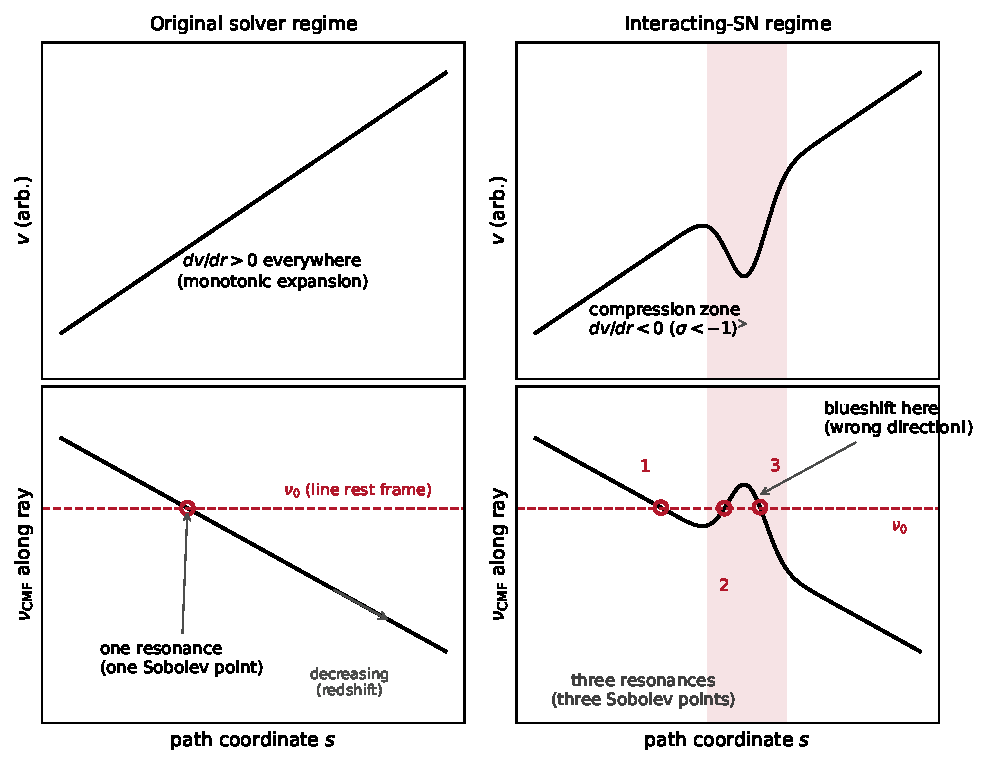
\includegraphics[width=\textwidth]{figures/fig_knop_crossings.pdf}
  \caption{Why monotonic velocity matters.  \emph{Top}: velocity
  profiles.  \emph{Bottom}: the comoving-frame frequency a fixed
  observer-frequency photon experiences as it travels along a ray.  In
  a monotonic outflow (left) the CMF frequency decreases smoothly and
  crosses each line rest frequency $\nu_0$ exactly once.  In a
  compression zone (right, shaded) the photon is \emph{blueshifted}:
  $\nu_{\rm CMF}$ turns around and crosses $\nu_0$ three times, creating
  three resonance points the original solver did not know how to
  handle.}
  \label{fig:crossings}
\end{figure}

\subsection{Why monotonicity was safe}

Two assumptions are baked into Eqs.~(\ref{eq:chihat}) and
(\ref{eq:shortchar}):
\begin{enumerate}[nosep]
  \item $\Gamma > 0$ everywhere, so $\hat\chi > \chi > 0$: the
        generalised opacity is positive, $\hat\tau$ is positive, and the
        solution factor $e^{-\hat\tau}$ attenuates light as physics
        demands.
  \item Photons only ever come from the previous (higher) frequency
        point, which the sweep has already computed.
\end{enumerate}
For a smooth, monotonically expanding atmosphere both hold
automatically, which is why the solver worked for decades.

%%------------------------------------------------------------------
\section{What a compression zone does to the original solver}
\label{sec:breaks}
%%------------------------------------------------------------------

A STELLA snapshot of an interacting supernova contains regions where the
fast shell material decelerates into the slower medium ahead, a
compression zone with $dv/dr < 0$, hence $\sigma < -1$ and $\Gamma < 0$.
Three things then go wrong at once:

\begin{enumerate}[nosep]
  \item \textbf{Negative optical depth.}  In Eq.~(\ref{eq:chihat}) the
        term $\Gamma/\Delta\ln\nu$ goes negative and can make
        $\hat\chi < 0$.  A negative opacity means $e^{-\hat\tau}$
        \emph{amplifies} light instead of attenuating it.  Intensities
        grow exponentially, go negative, and NaNs spread through the
        arrays.
  \item \textbf{Photons arrive from the wrong direction.}  Where the gas
        compresses, photons are blueshifted as they travel, so the
        photons arriving at frequency $\nu$ came from a \emph{lower}
        frequency: the \emph{next} point in the sweep, which has
        not been computed yet.  The solver nevertheless keeps using the
        previous point and gets the wrong answer even where it does not
        crash.
  \item \textbf{Multiple resonances.}  As Fig.~\ref{fig:crossings}
        (right) shows, a single observer-frame frequency can resonate
        with the same line at \emph{three} different locations along a
        ray.  A solver built for one Sobolev point per line per ray
        cannot represent this; and in the observer-frame transfer the
        bookkeeping index that walks the frequency grid could be sent
        in the wrong direction entirely (in the SN\,2024pba model the
        old one-directional index search was wrong at
        ${\sim}99.5\%$ of ray points).
\end{enumerate}

The old code already ``knew'' this could happen and protected itself by
\emph{clamping} $\sigma \ge -0.999$ before the formal solver saw it.
That prevented crashes, but it erased the compression zone from the
physics, which is precisely the feature we are trying to model.  It also
produced subtle wrongness rather than honest failure.

\begin{figure}[t]
  \centering
  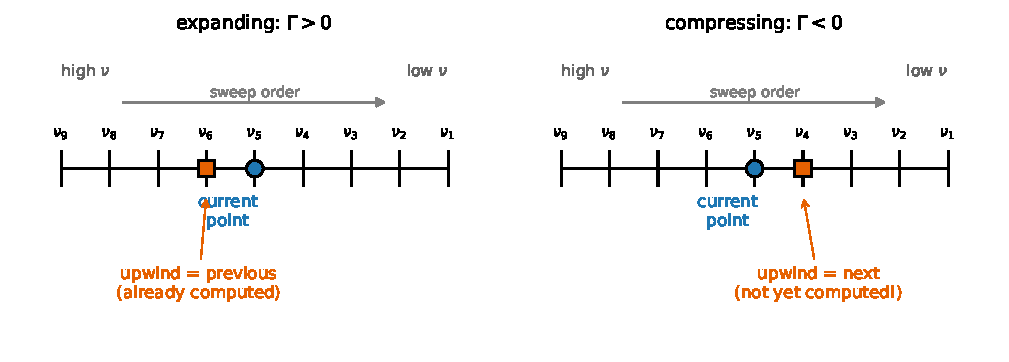
\includegraphics[width=\textwidth]{figures/fig_knop_upwind.pdf}
  \caption{The upwind-frequency choice on CMFGEN's frequency grid
  (sweeping high $\rightarrow$ low $\nu$).  In expanding gas
  ($\Gamma > 0$) photons redshift, so the photons at the current point
  came from the \emph{previous}, higher frequency, already computed.
  In a compression zone ($\Gamma < 0$) photons blueshift: they came
  from the \emph{next}, lower frequency, not yet computed in this
  sweep.  The Knop solver uses it anyway, from the previous
  \emph{iteration}'s stored values.}
  \label{fig:upwind}
\end{figure}

%%------------------------------------------------------------------
\section{The Knop et al.\ (2009) idea: separate strength from direction}
\label{sec:knop}
%%------------------------------------------------------------------

\citet{Knop2009} developed a formal solution for radiative transfer in
non-monotonic velocity fields (in the context of PHOENIX/3-D supernova
transfer).  The version implemented here follows the same logic.  The
central trick is to stop bundling two different things into one signed
number:

\begin{itemize}[nosep]
  \item the \emph{strength} of the velocity coupling (how rapidly
        photons drift in frequency) belongs in the opacity, and opacity
        must be positive;
  \item the \emph{direction} of the coupling (which neighbouring
        frequency photons arrive from) belongs in the source term,
        where a sign is perfectly legal.
\end{itemize}

\subsection{The new equations}

Equation~(\ref{eq:chihat}) is replaced by
\begin{align}
  \hat\chi &= \chi + \frac{|\Gamma|}{\Delta\ln\nu}
             &&\text{(magnitude only: always $>0$)}
             \label{eq:knop-chi}\\
  Q        &= \frac{\Gamma/\Delta\ln\nu}{\hat\chi}
             &&\text{(signed: keeps the direction)}
             \label{eq:knop-Q}\\
  S'       &= S + Q\,I_{\rm upwind},
  \label{eq:knop-src}
\end{align}
with the upwind neighbour chosen by the \emph{sign} of $\Gamma$:
\begin{equation}
  I_{\rm upwind} =
  \begin{cases}
    I_{\rm PREV} & \Gamma \ge 0 \quad\text{(expanding, as before)}\\
    I_{\rm NEXT} & \Gamma < 0 \quad\text{(compressing: Knop fix)} .
  \end{cases}
  \label{eq:upwind}
\end{equation}

The differential equation actually integrated, $dI/d\hat\tau = I - S'$,
is unchanged in form, so all the careful short-characteristics
machinery still applies.  What changed is that $\hat\tau$ can no longer
be negative, and the source function knows which way the ``river'' of
frequency coupling flows.

\subsection{The catch: the next frequency hasn't been computed yet}

CMFGEN sweeps from high to low frequency, so at the current point
$I_{\rm NEXT}$ (the lower-frequency neighbour) does not yet exist in
this sweep (Fig.~\ref{fig:upwind}).  The Knop scheme handles this with a
\emph{Gauss--Seidel iteration across ``great iterations''}, the same
philosophy as the $\Lambda$-iteration CMFGEN already uses:

\begin{enumerate}[nosep]
  \item On the first great iteration, set $I_{\rm NEXT} = 0$ at
        compressing points.  Crude, but stable: those points just get
        $S' = S$ (no frequency coupling) for one round.
  \item After each great iteration, store the computed intensities.
  \item On the next great iteration, use the stored values as
        $I_{\rm NEXT}$.
  \item Repeat until the stored and computed intensities agree.
\end{enumerate}

\subsection{Multiple resonance crossings}

Because $\nu_{\rm CMF}$ can turn around along a ray
(Fig.~\ref{fig:crossings}), one observer-frame frequency can hit the
same line at several depths.  The new solver integrates the ray
\emph{piecewise}: it marches along the ray, detects every sign change
of the frequency drift, and applies the short-characteristics step
segment by segment, so each resonance crossing is handled with the
correct local direction.  In the observer-frame module the bracketing
index $K$ is now allowed to move \emph{either way} along the frequency
grid (decrement first, then increment), rather than only ever
increasing.  This small change fixed the ${\sim}99.5\%$ index failure
rate on the SN\,2024pba model.

\subsection{Two $\sigma$ arrays: telling the truth selectively}
\label{sec:dual-sigma}

Much of CMFGEN's surrounding machinery (the moment equations, the BA
acceleration matrix, Ng extrapolation, Sobolev escape probabilities,
regridding) was written assuming $\sigma > -1$ and is unstable or
meaningless otherwise.  Rather than rewrite all of it, the solver keeps
two arrays:

\begin{center}
\begin{tabular}{lll}
\toprule
Array & Contents & Who sees it \\
\midrule
\code{SIGMA\_TRUE} & true, unclamped $d\ln v/d\ln r - 1$ &
   the Knop formal solver only \\
\code{SIGMA}       & clamped, $\ge -0.999$ &
   every other routine (stability) \\
\bottomrule
\end{tabular}
\end{center}

The formal solution, the place where the physics of the compression
actually enters the spectrum, sees the real velocity field.  The legacy
plumbing sees a safe, fake-monotonic version and keeps working.  A
useful analogy is a city map: the delivery driver (the formal solver)
gets the true map with all the one-way reversals; the traffic-planning
spreadsheet (the moment equations) gets a simplified map that never
reverses, so its assumptions still hold.

Because the moment equations cannot be trusted at $\sigma<-1$, the
non-monotonic path bypasses them: the Eddington factors that close the
system are computed directly from the ray moments
(\code{GET\_MOMS\_NON\_REL}, selected by \code{USE\_LAM\_ES=T}) instead
of from a tridiagonal moment solve.

\begin{figure}[t]
  \centering
  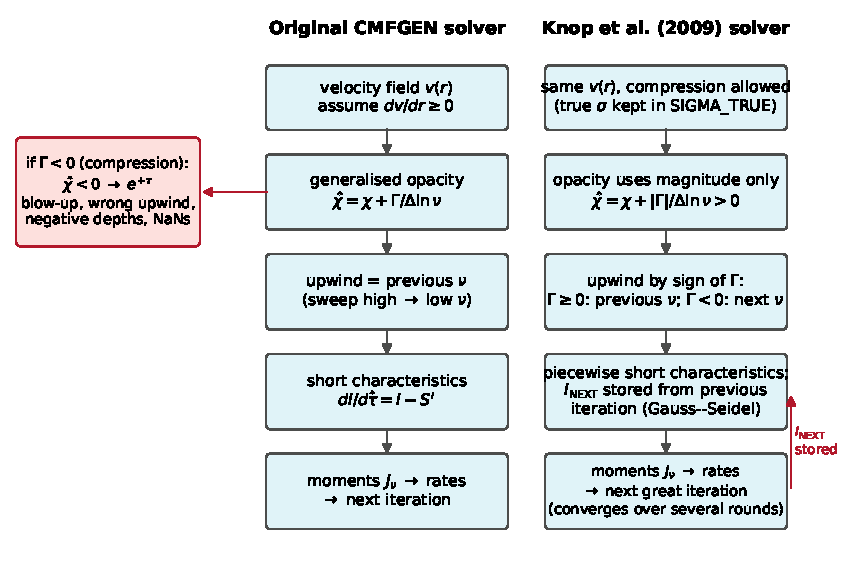
\includegraphics[width=0.95\textwidth]{figures/fig_knop_flowchart.pdf}
  \caption{The two formal solvers side by side.  Left: the original
  path, which implicitly requires $\Gamma>0$ (monotonic expansion) and
  fails in compression zones.  Right: the Knop et al.\ (2009) path: the
  opacity carries only $|\Gamma|$, the signed coupling $Q$ lives in the
  source function, the upwind neighbour is chosen by the sign of
  $\Gamma$, and the not-yet-computed $I_{\rm NEXT}$ is supplied from the
  previous great iteration.}
  \label{fig:flowchart}
\end{figure}

%%------------------------------------------------------------------
\section{A river analogy}
\label{sec:river}
%%------------------------------------------------------------------

For intuition, think of the frequency grid as a river flowing through a
row of towns (grid points), with photons as leaves on the water:

\begin{itemize}[nosep]
  \item \textbf{Normal flow} (expansion): the current carries leaves
        downstream, from high frequency to low.  Each town only needs to
        ask its upstream neighbour (already visited) how many leaves
        to expect.
  \item \textbf{Reversed stretch} (compression zone): the current runs
        \emph{backwards}.  Two bugs appear: the old formula counted the
        current's strength \emph{with its sign}, so a reversed current
        made the ``muddiness'' (opacity) negative, so leaves would
        multiply as they drift.  And the town now needs leaf counts from
        \emph{downstream}, a town not yet visited this round.
  \item \textbf{The Knop fix}: make the muddiness depend on the
        current's speed $|\Gamma|$, never its sign.  The river is always
        muddy.  Keep the sign separately to know which neighbour to ask.
        For the not-yet-visited downstream town, remember what it said
        \emph{last} round; over several rounds the remembered answers
        converge to the truth.
\end{itemize}

\begin{figure}[t]
  \centering
  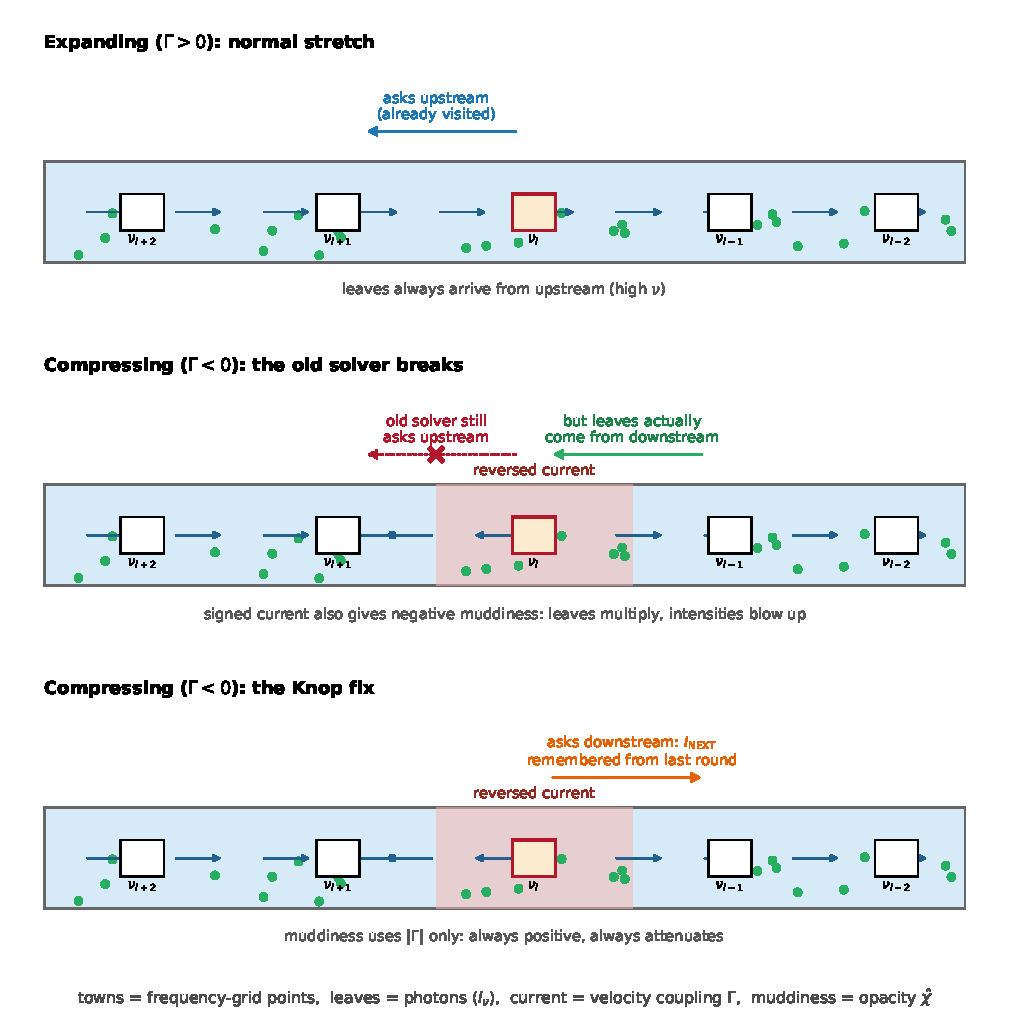
\includegraphics[width=\textwidth]{figures/fig_knop_river.pdf}
  \caption{The river analogy of \S\ref{sec:river}, drawn.  Each panel is
  a stretch of the frequency grid: towns are grid points, leaves are
  photons, the current is the velocity coupling $\Gamma$, and the
  muddiness of the water is the opacity $\hat\chi$.  \emph{Top:} in an
  expanding flow the current runs one way (high $\nu$ to low $\nu$,
  left to right), so each town asks the upstream neighbour it has
  already visited.  \emph{Middle:} in a compression zone the current
  reverses; the old solver still asks upstream and gets the wrong leaf
  count, while the signed coupling also makes the muddiness negative.
  \emph{Bottom:} the Knop solver asks downstream, using the previous
  iteration's stored intensities, and the muddiness depends only on
  $|\Gamma|$.}
  \label{fig:river}
\end{figure}

%%------------------------------------------------------------------
\section{What actually changed in the code}
\label{sec:code}
%%------------------------------------------------------------------

The solver is opt-in (\code{NON\_MONO\_SOLVER=T} in \code{VADAT}); a
monotonic model is completely unaffected.  The main pieces are:

\begin{center}
\begin{tabular}{p{5.4cm}p{9.2cm}}
\toprule
Piece & Role \\
\midrule
\code{FG\_J\_CMF\_NONMONO\_V1} &
  The new formal solver: Eqs.~(\ref{eq:knop-chi})--(\ref{eq:upwind}),
  piecewise integration across multiple crossings, Gauss--Seidel
  storage of $I_{\rm NEXT}$.  Replaces \code{FG\_J\_CMF\_V13} when
  enabled. \\
\code{SIGMA\_TRUE} &
  Parallel array carrying the unclamped velocity gradient; filled
  wherever the velocity law is set (hydro input, restart, observer
  module) and linearly interpolated to the ray grid. \\
Bidirectional $K$-index (\code{OBS\_FRAME\_SUB\_V9}) &
  Observer-frame bracketing index may now decrement \emph{or}
  increment, because in a compression zone the transformed frequency
  can move either way along the grid. \\
\code{USE\_LAM\_ES=T}, \code{GET\_MOMS\_NON\_REL} &
  Bypass the (unstable for $\sigma<-1$) moment-equation solve; take
  Eddington factors straight from the ray moments. \\
Forced \code{VADAT} settings &
  \code{GLOBAL\_LINE=BLANK}, \code{DO\_SOB\_LINES=F},
  \code{VEL\_LAW=11}, \code{PURE\_HUB=F} etc.\ are enforced so the
  non-monotonic path is self-consistent. \\
\bottomrule
\end{tabular}
\end{center}

A full routine-by-routine description lives in
\code{docs/cmfgen\_and\_nonmono\_solver.tex} and
\code{docs/CMFGEN\_NONMONO\_CHANGES.md}; this document is the
pedagogical version.

%%------------------------------------------------------------------
\section{Why SN\,2024pba needs this}
\label{sec:sn2024pba}
%%------------------------------------------------------------------

In our scenario the STELLA snapshot handed to CMFGEN contains a dense
SN\_B shell driving a forward shock at the shell/wind interface, with
radiatively heated (but unshocked) SN\_A ejecta beyond it.  The velocity
field across that interface is non-monotonic: the shocked gas
decelerates into the slower wind, producing exactly the compression
zones ($\sigma<-1$) that break the original solver.  Without the Knop
formal solution the options were both bad: crash, or clamp $\sigma$ and
silently erase the shock structure from the radiative transfer.  With
it, CMFGEN computes the spectrum on the \emph{actual} STELLA velocity
field: the shocks and compression zones survive into the formal
solution.

Two honest caveats remain.  First, stability is not accuracy: the BA
Jacobian still uses the clamped $\sigma$, so convergence in strongly
non-monotonic regions is approximate and slower.  Second, the
Gauss--Seidel coupling of $I_{\rm NEXT}$ needs several great iterations
to converge, so non-monotonic runs need more iterations before their
spectra are trustworthy.

\begin{thebibliography}{}
\bibitem[Hillier \& Miller(1998)]{Hillier1998}
  Hillier, D.~J., \& Miller, D.~L.\ 1998, ApJ, 496, 407
\bibitem[Knop et al.(2009)]{Knop2009}
  Knop, S., Hauschildt, P.~H., \& Baron, E.\ 2009, A\&A, 501, 913
\bibitem[Ng(1974)]{Ng1974}
  Ng, K.~C.\ 1974, J.\ Chem.\ Phys., 61, 2680
\bibitem[Rybicki \& Hummer(1991)]{RybickiHummer1991}
  Rybicki, G.~B., \& Hummer, D.~G.\ 1991, A\&A, 245, 171
\end{thebibliography}

\end{document}
